% SynAthlete-AIoT in the IEEE Access template (ieeeaccess.cls; upload it with this file).
% Every number comes from generated/*.tex, written by `python tasks.py paper-figures` from the
% experiments/**/metrics.json files (AGENTS.md invariant 1). Do not type numbers by hand.
\documentclass{ieeeaccess}
\usepackage{cite}
\usepackage{amsmath,amssymb,amsfonts}
\usepackage{graphicx}
\usepackage{textcomp}
\usepackage{booktabs}
\usepackage{xspace}
\usepackage{url}
% generated by src/paper/figures.py: do not edit
\newcommand{\canaryAuc}{0.498 (day) and 0.513 (week)\xspace}
\newcommand{\explainSummary}{Explanation checks: n/a.\xspace}
\newcommand{\fusedAuc}{n/a\xspace}
\newcommand{\fusedPrAuc}{n/a\xspace}
\newcommand{\injuryAucRange}{0.58--0.63\xspace}
\newcommand{\labelFreeAuc}{0.584 (day) and 0.589 (week)\xspace}
\newcommand{\lockboxSummary}{Pending the evaluation freeze.\xspace}
\newcommand{\lovdalRunners}{74\xspace}
\newcommand{\pamapRealFone}{0.632\xspace}
\newcommand{\reproDayAuc}{0.617 (95\% CI 0.573--0.664)\xspace}
\newcommand{\tiersReduction}{n/a\xspace}


\begin{document}
\history{Date of publication xxxx 00, 0000, date of current version xxxx 00, 0000.}
\doi{10.1109/ACCESS.2026.DOI}

\title{SynAthlete-AIoT: An Honest, Explainable AIoT Pipeline for Athlete Injury-Risk
Prediction with Synthetic Wearable Data}
\author{\uppercase{[Author names to be added]}\authorrefmark{1}}
\address[1]{[Department], SRM Institute of Science and Technology, India}
\tfootnote{[Support and acknowledgment information to be added.]}

\markboth
{Author \headeretal: SynAthlete-AIoT: Honest, Explainable AIoT Injury-Risk Prediction}
{Author \headeretal: SynAthlete-AIoT: Honest, Explainable AIoT Injury-Risk Prediction}

\corresp{Corresponding author: [Name] (e-mail: [address]).}

\begin{abstract}
Wearable artificial-intelligence-of-things (AIoT) systems promise early warning of athlete
injuries, but published frameworks often stop at the design stage, and reported accuracies can
be inflated by evaluation shortcuts such as data leakage. We implement a complete pipeline:
class-conditional generators for synthetic wearable data, simulated edge, fog and cloud tiers,
a fused sequence-plus-tabular injury model, explanations checked by faithfulness tests, and a
coach dashboard. We evaluate it under a pre-registered, person-level protocol on real injury
data from 74 competitive runners, with ten runners sealed as a final test that was opened once
after an evaluation freeze. Learned models predict injuries only modestly above chance
(ROC-AUC \injuryAucRange{} over five development rounds), and the declared fused model kept
its level on the sealed runners. A rebuild of a published bagged gradient-boosting method passed
a pre-registered sanity check. Three generators and classic augmentation were judged against
criteria fixed before any run; none produced data that a real-versus-synthetic classifier could
not separate, and synthetic injury examples gave no measurable gain. Processing at the edge sent
\tiersReduction{} less data to the cloud for the wearable stream. Explanations passed deletion,
randomisation and stability tests in every round. We report every model, failures included,
and release the protocol and code.
\end{abstract}

\begin{keywords}
Athlete monitoring, data leakage, edge computing, explainable artificial intelligence,
injury prediction, Internet of Things, synthetic data, wearable sensors
\end{keywords}

\titlepgskip=-15pt

\maketitle

\section{Introduction}
\label{sec:introduction}
\PARstart{C}{oaches} need to see injury risk building up over days, not in single snapshots.
AIoT designs for athlete health propose wearables with edge, fog and cloud processing, but the
prediction and explanation layers are often left unimplemented. Public data
make the problem harder: no public dataset pairs high-frequency physiological streams with real
injury outcomes. Daily training logs with real injuries do exist~\cite{lovdal2021,lovdal2021data},
while wearable datasets with rich physiology have no injury labels~\cite{reiss2012,schmidt2018}.
We therefore treat the two kinds of data as two tracks with separate roles: injury evidence comes
only from real injury labels, and the wearable streams drive the IoT tiers and the generators.

A second problem is evaluation. Injury events are rare, models are tuned on small cohorts, and
preprocessing can quietly use test labels; such leakage inflates results~\cite{kapoor2023}, and
model selection outside the test loop biases them~\cite{varma2006,cawley2010}. We fixed the
protocol, the model list, the tuning budget and every pass mark in writing before the first run,
and we kept ten runners sealed until the code was frozen.

\textbf{Contributions.}
\begin{enumerate}
\item An end-to-end, open AIoT pipeline in which each component and each dataset has one
explicit, honest role.
\item A pre-registered, person-level evaluation protocol with a sealed final test opened once,
a leak alarm, runner-level uncertainty and paired comparisons.
\item A rebuild of a published injury-prediction method that passed a pre-registered sanity
check, and a label-free variant that a deployed system could actually use.
\item A generator comparison (TimeGAN, WGAN-GP, TimeVAE and classic augmentation) judged against
criteria fixed before any run, on two wearable datasets and as injury-data augmentation.
\item Explanations checked by deletion, model-randomisation and stability tests and against a
list of expectations written before running, rather than assumed.
\end{enumerate}

\section{Related Work}
\subsection{Injury Prediction}
L\"ovdal et al.\ predicted injuries of competitive runners from daily training logs with bagged
gradient-boosted trees~\cite{lovdal2021,chen2016}. Tree ensembles remain strong on tabular
data~\cite{grinsztajn2022,breiman2001,prokhorenkova2018}, and recurrent networks read days in
order~\cite{cho2014}. Temporal convolutional networks offer another sequence
model~\cite{bai2018}.

\subsection{Synthetic Time Series}
TimeGAN~\cite{yoon2019}, WGAN-GP~\cite{gulrajani2017} and TimeVAE~\cite{desai2021} generate
sequences; classic augmentation such as jitter, scaling and time-warping~\cite{um2017} is a
strong baseline. Synthetic data are useful only if they are realistic, useful for training and
do not copy real records.

\subsection{Explanations}
SHAP~\cite{lundberg2017} and integrated gradients~\cite{sundararajan2017} attribute predictions
to inputs. Sanity checks show that attributions must be tested rather than
assumed~\cite{adebayo2018}; attention weights alone are not explanations.

\subsection{Evaluation}
With rare events, PR-AUC is more informative than ROC-AUC~\cite{saito2015,davis2006};
calibration and decision curves complete the picture~\cite{vancalster2019,vickers2006}.
Resampling whole people rather than rows gives honest uncertainty~\cite{field2007}.

\section{Data and Roles}
Table~\ref{tab:data} lists every dataset and its single role. Injury claims come only from the
L\"ovdal runner logs~\cite{lovdal2021data}: \lovdalRunners{} runners, a day file (7 days
$\times$ 10 features) and a week file (3 weeks $\times$ 22 features plus 3 relative changes).
PAMAP2~\cite{reiss2012} provides the wearable stream (heart rate and three accelerometers, 25~Hz,
5.12-s windows); WESAD~\cite{schmidt2018} tests generator generalisation; Sport DB 2.0 checks
heart-rate realism; SoccerMon~\cite{midoglu2024} and PMData are exploratory. Datasets of unknown
origin appear only as labelled demonstrations. Synthetic data is never evidence about real
injuries, and the wearable participants are different people from the runners.
\begin{table}[t]\centering\caption{Datasets and their single role}\label{tab:data}
\footnotesize\begin{tabular}{p{2.6cm}p{1.2cm}p{3.6cm}}\toprule
Dataset & Origin & Role \\\midrule
Lövdal runners (74 runners, 7 years of daily logs) & real & the only injury evidence: baselines, combined model, explanations, coach view \\
Kaggle 'Injury Prediction for Competitive Runners' & real (copy) & byte-identical copy of Lövdal: no separate role \\
PAMAP2 (9 people, wearable sensors) & real & edge sensor stream, activity recognition, generator training and fidelity \\
WESAD (15 people, wrist sensors) & real & second dataset for generator generalisation \\
Sport DB 2.0 (55 heart-rate recordings) & real & heart-rate realism check and second edge stream \\
SoccerMon, PMData & real & exploratory only (Track C), never main evidence \\
SIRP-600 & unknown origin & demo only: shows the SHAP code runs \\
ziya07 wearable & unknown origin & demo only: dashboard demo stream \\
\bottomrule\end{tabular}\end{table}


\section{Evaluation Protocol}
\subsection{Splits}
All splits are by person. The ten most recently joined runners form a sealed final test, opened
once after an evaluation freeze through a guarded loader that checks an annotated, pushed tag,
an unchanged code tree and a single frozen commit, and logs every opening. The other 64 runners
form five development rounds; in each, settings, Platt calibration, the alert level and early
stopping use that round's validation runners only, and its test runners are scored once.

\subsection{Scoring}
The headline metric is PR-AUC (average precision) next to the injury rate, its chance level,
with ROC-AUC for comparison with the literature. The alert level minimises
$|\mathrm{sensitivity}-\mathrm{specificity}|$ on validation runners. Alert results are reported
for the sealed final test; per-round calibration and alert results are kept in the result files.

\subsection{Tuning}
Eight settings per model and round by seeded random search~\cite{bergstra2012}, written before
the first run; the chosen setting is refit with three seeds.

\subsection{Leakage Controls}
One z-score scaler fitted on training runners only; no identity, date or own-history inputs (in
this dataset, a runner's own event history reveals the label); a shuffled-label alarm whose
ROC-AUC stayed at \canaryAuc{}~\cite{ojala2010}; and independent code reviews before the freeze
and before reporting.

\subsection{Uncertainty and Comparisons}
Runner-level cluster bootstrap within test groups (2,000 resamples)~\cite{field2007}. Models are
compared in pre-declared pairs on the same rows; a difference counts only when its interval
excludes zero, and the intervals are not adjusted for multiple comparisons.

\section{Methods}
\subsection{Baselines}
Constant risk, an uncoupled ACWR-style rule~\cite{lolli2019}, logistic regression, random forest,
CatBoost and a GRU. The L\"ovdal bagged gradient-boosting method was rebuilt twice: as an exact
copy, including its normalisation step that reads the labels, run once as a sanity check on
stand-in runners; and as a label-free variant, compared on the five rounds.

\subsection{Fused Model}
A sequence arm (GRU, LSTM or TCN~\cite{bai2018}) on day sequences and a tabular arm (random
forest or CatBoost) on week features, chosen per round on validation runners, are combined by
logistic regression trained on out-of-fold arm predictions grouped by runner, so that the
combiner never sees a prediction made by a model that trained on that runner. The calibrated
output is shown as a 0--100 risk score (its percentile among validation events). The fused model
was declared in advance as the model for the sealed test.

\subsection{Generators}
Class-conditional TimeGAN, WGAN-GP and TimeVAE are trained only on each round's training people,
with settings chosen by validation train-on-synthetic-test-on-real (TSTR) macro-F1 (WGAN-GP: one
declared setting, untuned), plus classic augmentation. They are judged by a real-versus-synthetic
classifier, TSTR, autocorrelation and correlation errors and a nearest-record privacy test, all
with pass marks fixed in advance.

\subsection{Edge, Fog and Cloud Tiers}
Edge (a reflex check and the activity network per window), fog (session summaries) and cloud (the
daily injury model) run as separate processes joined by queues. We compare the bytes that reach
the cloud and the decision latency with a cloud-only design that sends every raw window.

\subsection{Explanations}
TreeSHAP on the tabular arm, integrated gradients on the sequence arm, an explanation-only
attention model always shown next to integrated gradients, and one-dimensional Grad-CAM on the
activity network; all are checked by deletion, model-randomisation and stability tests with
thresholds fixed in advance, and each risk score gets a plain-language reason sentence.

\section{Results}
\begin{table}[t]\centering\caption{Injury prediction, mean $\pm$ SD over five development rounds (chance PR-AUC $\approx$ injury rate)}\label{tab:injury}
\footnotesize\begin{tabular}{llcc}\toprule
Model & File & PR-AUC & ROC-AUC \\\midrule
Constant risk & day & 0.013 $\pm$ 0.000 & 0.500 $\pm$ 0.000 \\
Constant risk & week & 0.013 $\pm$ 0.000 & 0.500 $\pm$ 0.000 \\
ACWR-style rule & week & 0.015 $\pm$ 0.001 & 0.540 $\pm$ 0.021 \\
Logistic regression & day & 0.022 $\pm$ 0.004 & 0.626 $\pm$ 0.019 \\
Logistic regression & week & 0.020 $\pm$ 0.004 & 0.621 $\pm$ 0.029 \\
Random forest & day & 0.019 $\pm$ 0.002 & 0.603 $\pm$ 0.024 \\
Random forest & week & 0.022 $\pm$ 0.007 & 0.614 $\pm$ 0.042 \\
CatBoost & day & 0.021 $\pm$ 0.004 & 0.598 $\pm$ 0.043 \\
CatBoost & week & 0.019 $\pm$ 0.002 & 0.606 $\pm$ 0.028 \\
GRU & day & 0.023 $\pm$ 0.006 & 0.631 $\pm$ 0.009 \\
L\"ovdal, label-free & day & 0.017 $\pm$ 0.003 & 0.584 $\pm$ 0.044 \\
L\"ovdal, label-free & week & 0.021 $\pm$ 0.006 & 0.589 $\pm$ 0.066 \\
\textbf{Fused} & shared & 0.022 $\pm$ 0.003 & 0.609 $\pm$ 0.024 \\
\bottomrule\end{tabular}\end{table}

\subsection{Injury Prediction}
Table~\ref{tab:injury} shows every model. The leak alarm stayed at chance. Learned models reach
ROC-AUC \injuryAucRange{}; only a few pre-declared pairs differ clearly
(Table~\ref{tab:compare}). The fused model reaches ROC-AUC \fusedAuc{} and PR-AUC \fusedPrAuc{}.
The exact copy of the published method passed its pre-registered sanity check (day-file ROC-AUC
\reproDayAuc{}); the label-free variant reaches ROC-AUC \labelFreeAuc{}. The two were scored on
different runners, so the effect of the label-reading step was not measured head-to-head.

\begin{figure}[t]
\centering
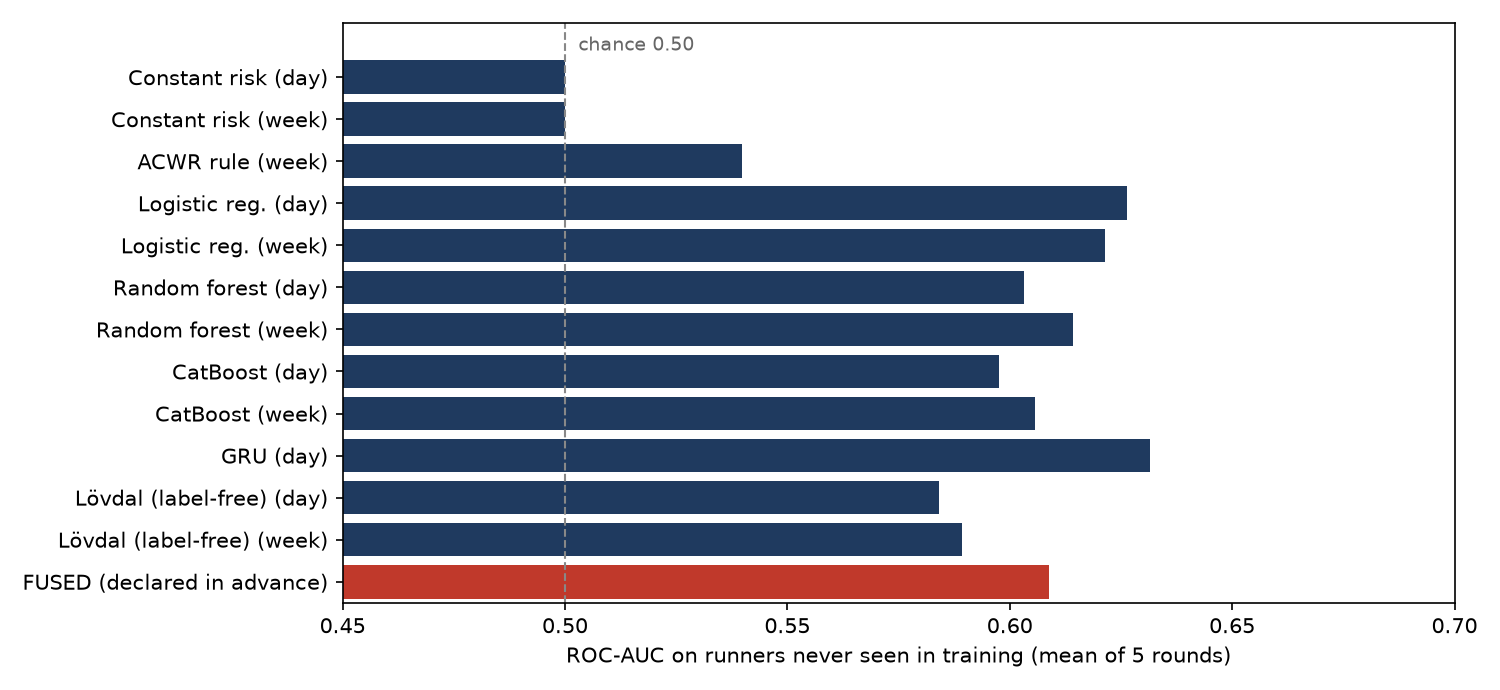
\includegraphics[width=\columnwidth]{injury_auc.png}
\caption{ROC-AUC of every injury model on runners never seen in training (mean of five
development rounds). The fused model is highlighted because it was declared in advance, not
because it was best.}
\label{fig:injury}
\end{figure}

\subsection{Sealed Final Test}
\lockboxSummary{} The development and sealed-test results agree, which indicates that the
development results were not over-tuned. With ten runners, ranking models on the sealed test
is not possible.

\subsection{Model Comparisons}
\begin{table}[t]\centering\caption{Paired differences (5-round mean, runner bootstrap 95\% interval, 2,000 resamples)}\label{tab:compare}
\footnotesize\begin{tabular}{lcc}\toprule
Comparison & $\Delta$ PR-AUC & $\Delta$ ROC-AUC \\\midrule
\multicolumn{3}{c}{n/a} \\
\bottomrule\end{tabular}\end{table}

Table~\ref{tab:compare} gives paired differences with runner-bootstrap intervals. Against the
label-free variant, logistic regression and the GRU on the day file are clearly better on both
metrics, and CatBoost on the day file on PR-AUC only; constant risk and the ACWR-style rule are
clearly worse. The fused model's gain over its sequence arm is borderline on ROC-AUC and absent
on PR-AUC; it shows no gain over its tabular arm.

\subsection{Synthetic Data}
\begin{table}[t]\centering\caption{Generators on PAMAP2 (4 rounds): discriminative accuracy (0.5 = indistinguishable), TSTR and real+synthetic macro-F1, pre-registered criteria passed}\label{tab:gen}
\footnotesize\begin{tabular}{lcccc}\toprule
Generator & Disc.\ acc. & TSTR & Real+syn. & Passed \\\midrule
\multicolumn{5}{c}{n/a} \\
\bottomrule\end{tabular}\end{table}

Table~\ref{tab:gen} compares the generators with real-data training (real-only macro-F1
\pamapRealFone{}). \wesadSummary{} \augmentSummary{}

\subsection{Edge, Fog and Cloud Tiers}
\begin{table}[t]\centering\caption{Edge--fog--cloud vs cloud-only (simulated on one computer)}\label{tab:tiers}
\footnotesize\begin{tabular}{llrr}\toprule
Stream & Mode & Bytes into cloud & Median decision (ms) \\\midrule
\multicolumn{4}{c}{n/a} \\
\bottomrule\end{tabular}\end{table}

Processing at the edge reduced the data sent to the cloud by \tiersReduction{} for the wearable
stream (Table~\ref{tab:tiers}). Every tier is set up before the first window and windows are
sent at a steady pace, so latency is decision time; on one computer there is no network delay,
so it compares processing only.

\subsection{Explanations}
\explainSummary{}

\section{Discussion and Limitations}
Training logs alone carry little warning before an injury: honest models are only modestly
better than chance, and the alert level that balances sensitivity and specificity raises many
false alarms. This is why we report every model and kept the final test sealed until the end.
The dataset's authors removed healthy days close to injuries, so alert rates are not daily rates
and net benefit is not clinical utility. The sealed test has only ten runners, and its interval
understates the uncertainty. The tiers are simulated on one computer, and the wearable streams
come from different people than the runners: they demonstrate the system, not injury evidence.
The generators did not produce data that a classifier could not separate from real data, so
synthetic data was used for training only.

\section{Conclusion}
We implemented and honestly evaluated a complete explainable AIoT pipeline for athlete injury
risk. Under a pre-registered, person-level protocol with a sealed final test, injury risk from
training logs is predictable only modestly, the edge tier sharply reduces cloud traffic, and
explanations pass faithfulness tests. The protocol, code and all results, including negative
ones, are released for reuse.

\section*{AI-Use Statement}
AI coding assistants helped write code and text under human direction; every AI contribution is
logged in the project's AI log, every number is produced by code, and all claims were checked by
the authors.

\bibliographystyle{IEEEtran}
\bibliography{refs}

\EOD

\end{document}
